\section{Scatter Plot: Discovering Relationships Between Two Variables}

A scatter plot is a type of graph that shows the relationship between two numerical variables. Each point on the plot represents one observation in your data, defined by its values on two axes.

\subsection*{Key Concepts: Let’s Explore}

\begin{enumerate}
    \item \textbf{Two Variables: X and Y} \\
    Think about situations where two quantities vary together:
    \begin{itemize}
        \item Hours studied vs. test scores
        \item Height vs. weight
        \item Temperature vs. ice cream sales
    \end{itemize}
    Can you think of three more examples where one thing might change as another?

    \item \textbf{Each Point = One Observation} \\
    In a scatter plot, each dot represents one observation from your dataset. Its position is determined by:
    \begin{itemize}
        \item Its value on the x-axis (horizontal)
        \item Its value on the y-axis (vertical)
    \end{itemize}

    \item \textbf{Patterns: Relationships or Trends} \\
    Scatter plots help us see relationships between variables:
    \begin{itemize}
        \item Positive relationship: As X increases, Y tends to increase
        \item Negative relationship: As X increases, Y tends to decrease
        \item No clear relationship: The points appear scattered
    \end{itemize}
    If your plot shows points climbing upwards, what might that suggest?

    \item \textbf{Clusters, Outliers, and Spread} \\
    Scatter plots also reveal:
    \begin{itemize}
        \item Clusters: Groups of similar points 
        \item Outliers: Distant or unusual points
        \item Spread: How widely points are distributed
    \end{itemize}

    \item \textbf{Line of Best Fit (Trend Line)} \\
    Sometimes we add a trend line (or regression line) to summarize the general direction of the relationship.
\end{enumerate}

\subsection*{Let’s Try This!}

We have our daily climate dataset. We want to explore how the Humidity and Temperature vary. We can observe this relation with scatter plots.

\paragraph{Relation between humidity and temperature above 2m}

\begin{verbatim}
xyplot(Humidity_2m ~ Temp_2m, data = df_climate,
       main = "Humidity vs. Temperature" ,xlab = "Temperature (°C)",
       ylab = "Humidity (%)", col = "blue",
       panel = function(x, y) {panel.xyplot(x, y)
           panel.abline(lm(y ~ x), col = "red", lwd = 2) #linear trend line
       })  # point color
\end{verbatim}

% Figure here -------------------------
\begin{figure}[h]
\centering
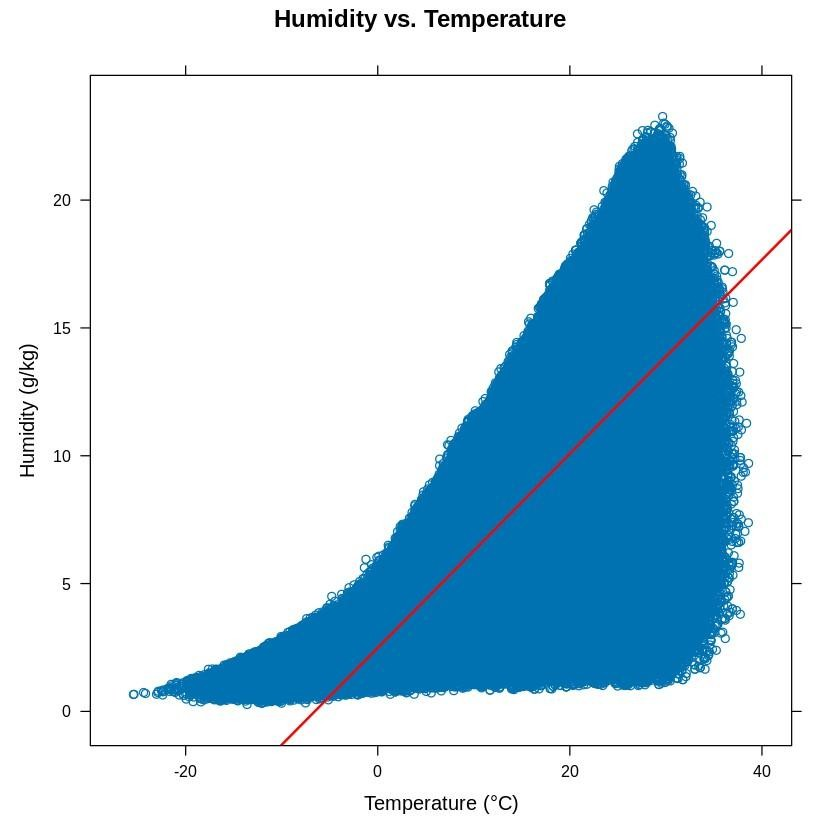
\includegraphics[width=0.5\textwidth]{figures/scatter1.jpg}
\caption{Humidity vs Temperature}
\end{figure}

\subsection*{Analyzing the Relationship Between Wind Speed and Precipitation}

To explore how wind speed at 10 meters (WindSpeed\_10m) relates to precipitation levels (Precip), we use a scatter plot.

\paragraph{Why a Scatter Plot?}

A scatter plot is a two-dimensional graph that displays individual data points for two variables. It helps us see:
\begin{itemize}
    \item Whether there is a relationship or trend between the two variables.
    \item The direction of the relationship (positive, negative, or none).
    \item How closely the points follow a pattern (correlation).
\end{itemize}

In our case, each point represents a day (or observation) with its wind speed on the x-axis and precipitation amount on the y-axis.

\paragraph{R Code: Creating a Scatter Plot with a Trend Line}

\begin{verbatim}
ggplot(climate_data, aes(x = WindSpeed_10m, y = Precip)) +
  geom_point(color = "blue") +
  geom_smooth(method = "lm", color = "red", se = FALSE) +
  labs(title = "Relationship Between Wind Speed and Precipitation",
       x = "Wind Speed (km/h)", y = "Precipitation (mm)") +
  theme_minimal()
\end{verbatim}

% Figure here--------------------------
\begin{figure}[h]
\centering
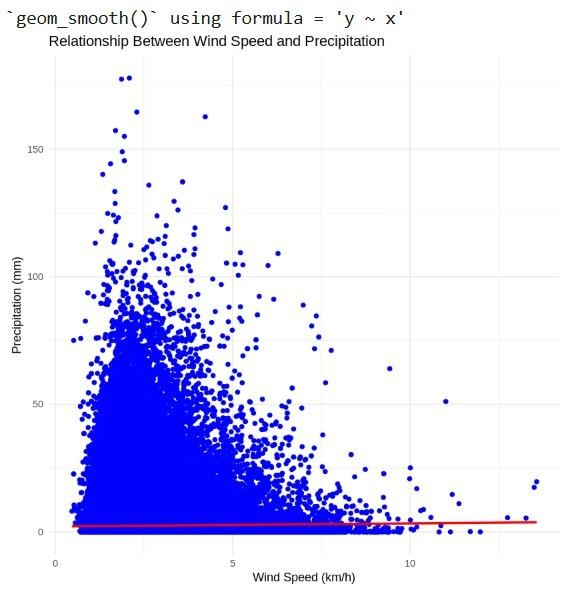
\includegraphics[width=0.5\textwidth]{figures/scatter2.jpg}
\caption{Wind Speed vs Precipitation}
\end{figure}

\paragraph{Explanation:}
\begin{itemize}
    \item \texttt{geom\_point()}: Plots each data point (blue dots).
    \item \texttt{geom\_smooth(method = "lm")}: Adds a red trend line using linear regression.
    \item \texttt{labs()}: Sets the title and axis labels for clarity.
    \item \texttt{theme\_minimal()}: Uses a clean, minimal background.
\end{itemize}

\paragraph{Interpretation:} 

If the red line slopes upward, it indicates that wind speed tends to increase as precipitation increases (a positive relationship). If the slope is downward, it indicates a negative relationship. A flat line suggests no clear relationship between the two variables.

\textit{Activity: Look at the scatter plot—do the points follow a clear upward or downward trend? Are they tightly clustered around the line, or widely scattered? What does this tell you about how wind and rain might interact in this climate?}
